The following sources of uncertainty are considered for the data-driven background estimation of the $\tau$ fakes in the $\tau_{lep}\tau_{had}$ channel.

\begin{itemize}
\item The statistical uncertainty on the $t\bar{t}$ fake factor (considered conservatively as a single variation)
\item The statistical uncertainty on the QCD fake factor (considered conservatively as a single variation)
\item The statistical uncertainty on the fraction of QCD (considered conservatively as a single variation)
\item The uncertainty on the estimation of non-$t\bar{t}$ backgrounds, taken to be 30\% to well cover potential modelling uncertainties)
\item The uncertainty on the modelling of the $t\bar{t}$ background, taken from the comparison between before and after applying $t\bar{t}$ reweighting. 
         The FF comparison with \ttbar-reweighting vs. no-\ttbar-reweighting is shown in Fig. \ref{fig:FFRW} for a demonstration of this uncertainty.  
\item  Given the small impact of rQCD on the fake estimate and the necessity of using MC to determine it, we have introduced a conservative systematic uncertainty for rQCD to range from 0 to 1 in the fit.
\end{itemize}

\begin{figure}[!h]
\centering
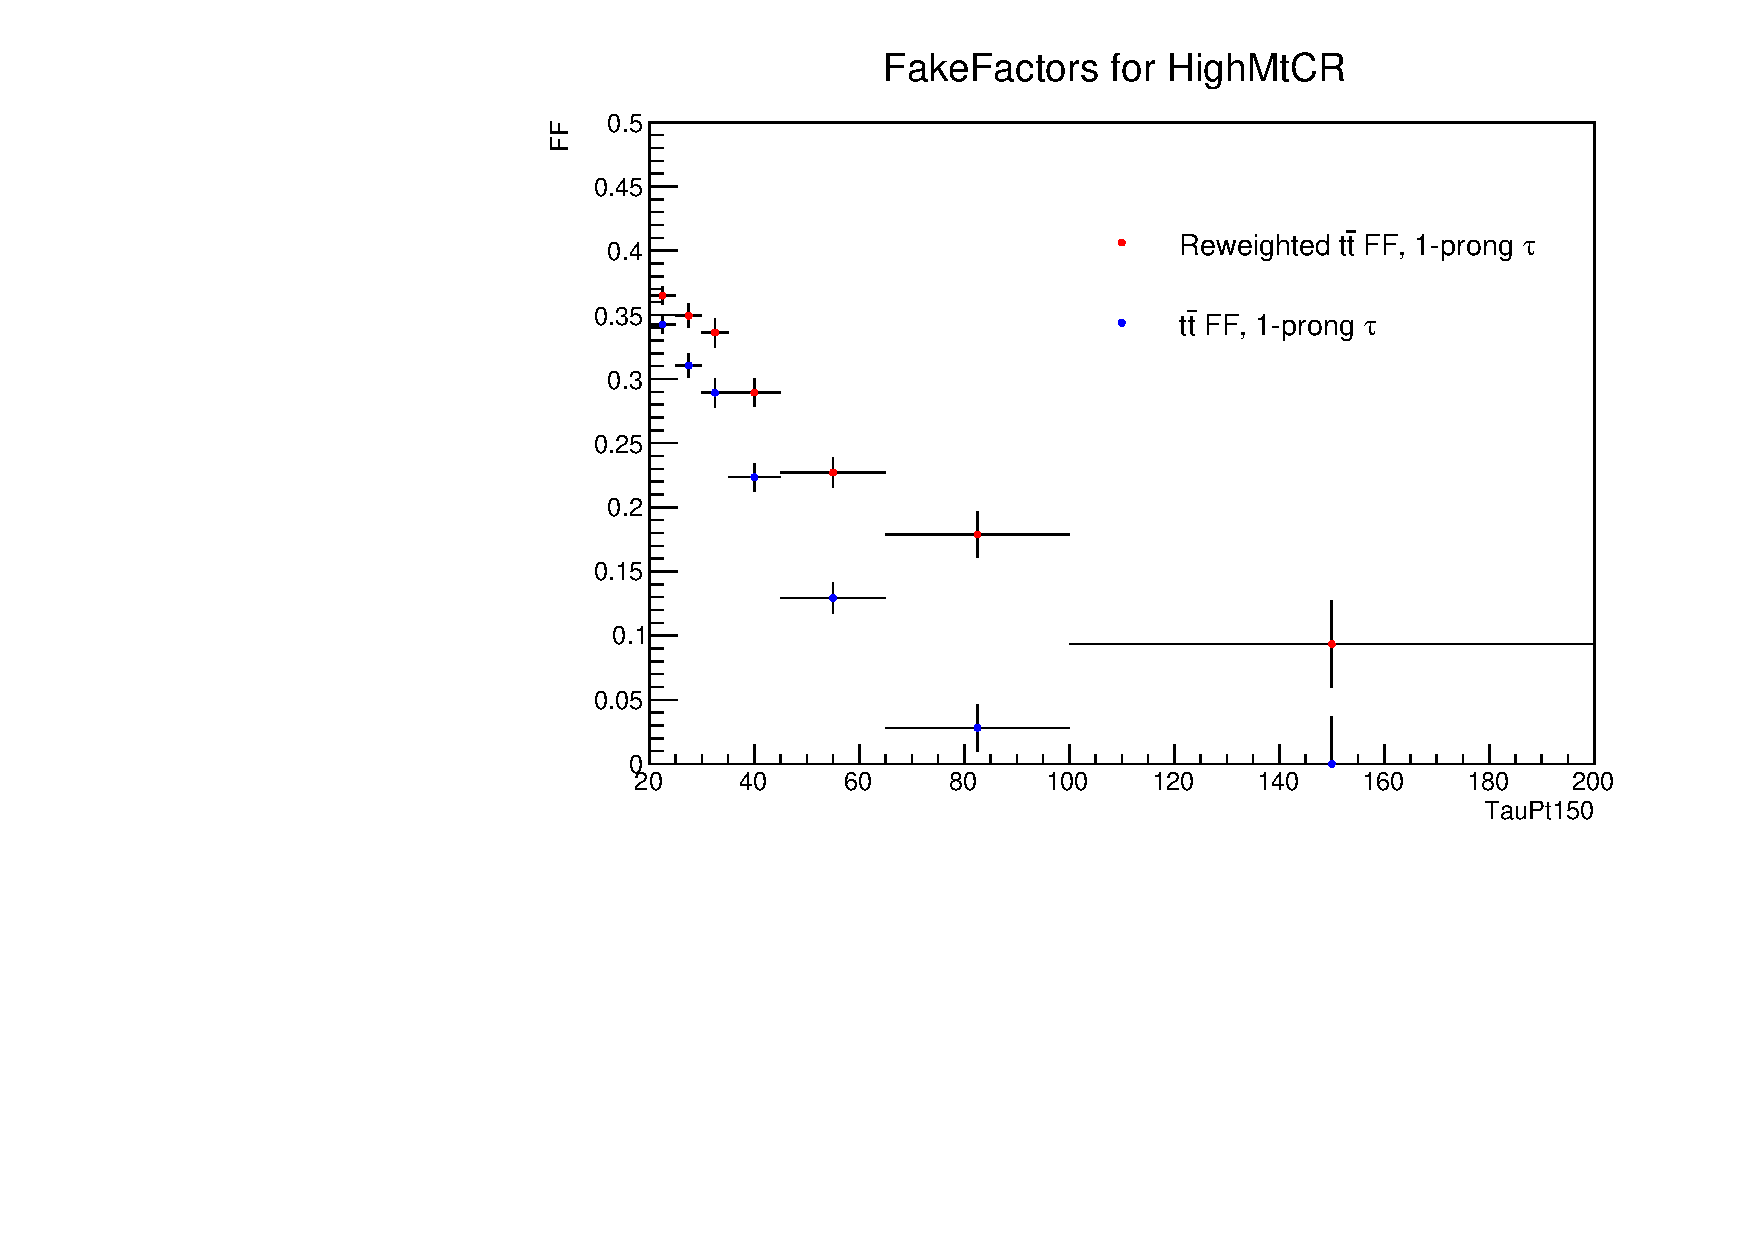
\includegraphics[width=.45\textwidth]{figures/systs/datadriven_lephadfakes/SLT/FFRWUnc_1prong_SLT.pdf}
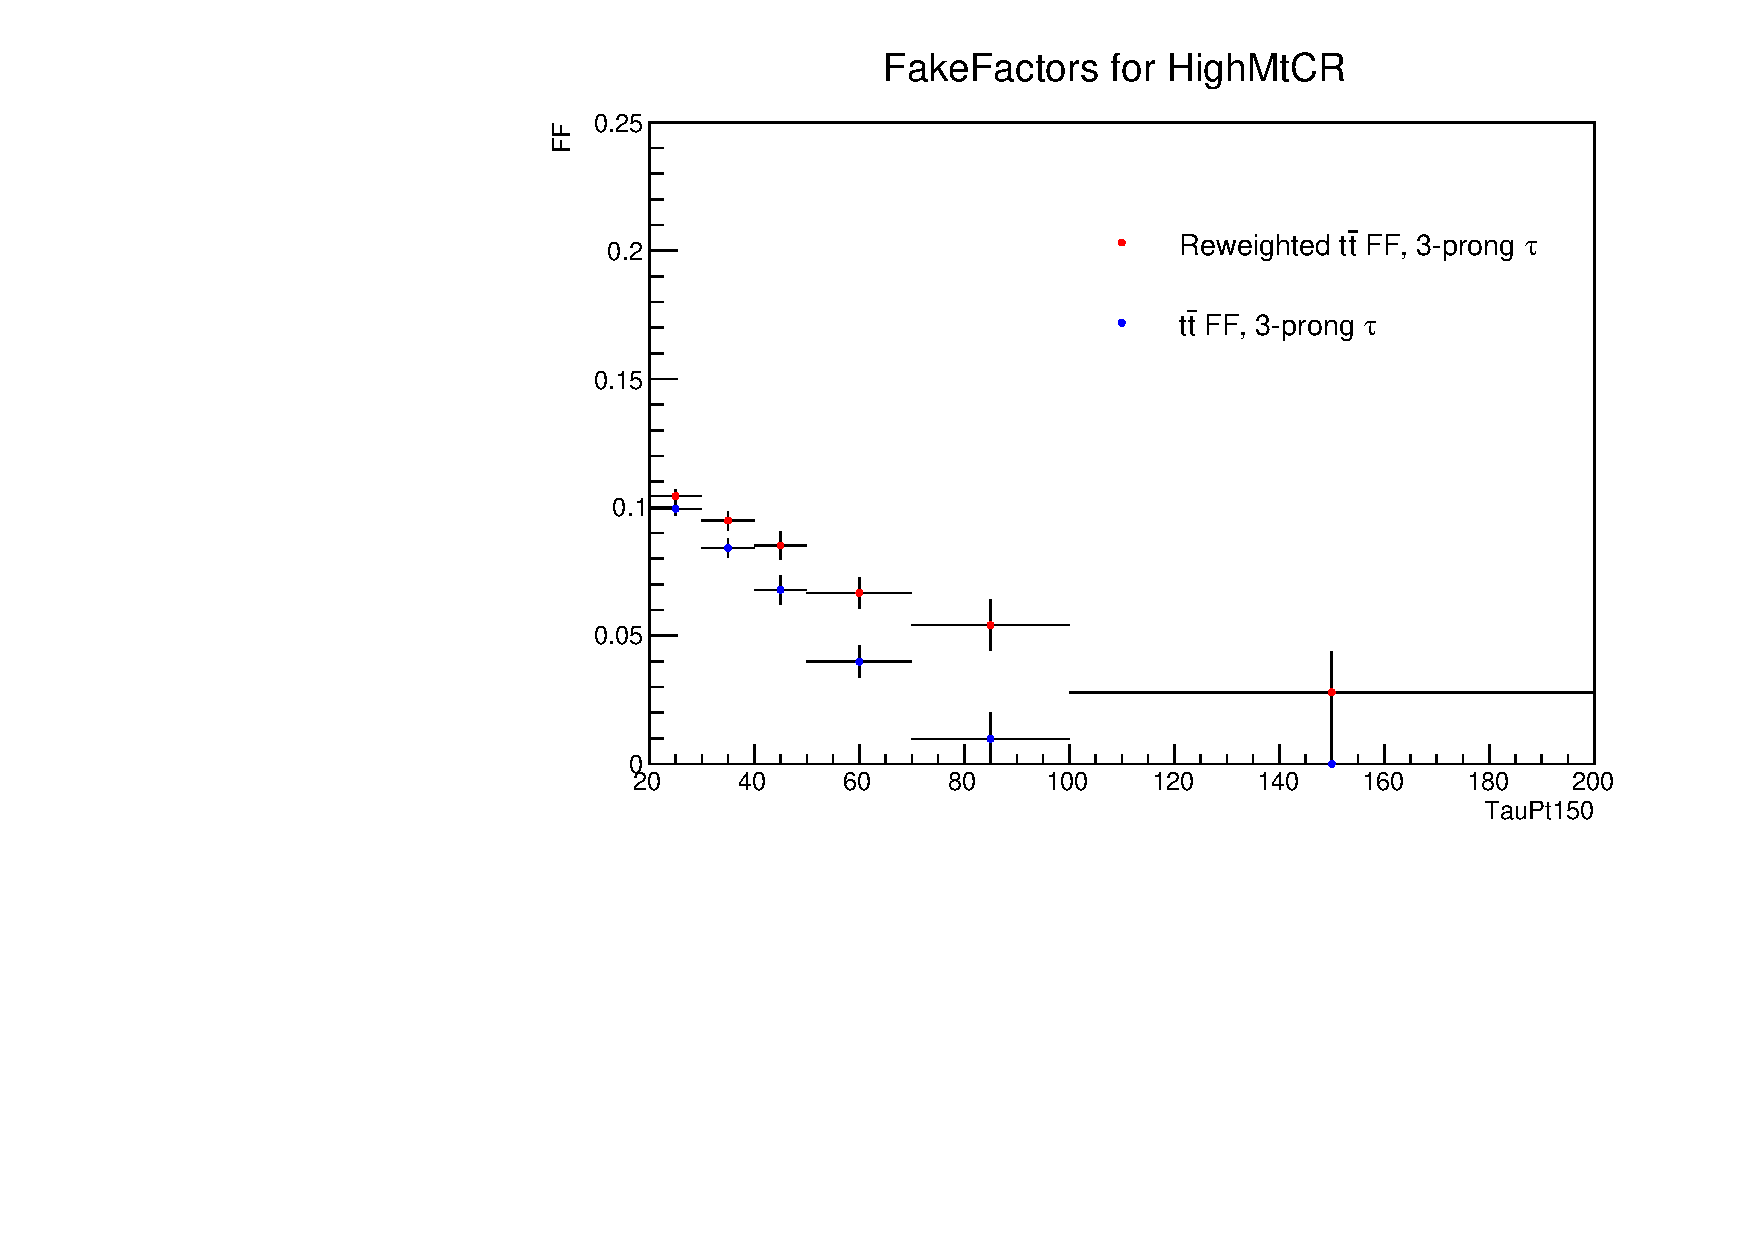
\includegraphics[width=.45\textwidth]{figures/systs/datadriven_lephadfakes/SLT/FFRWUnc_3prong_SLT.pdf} \\
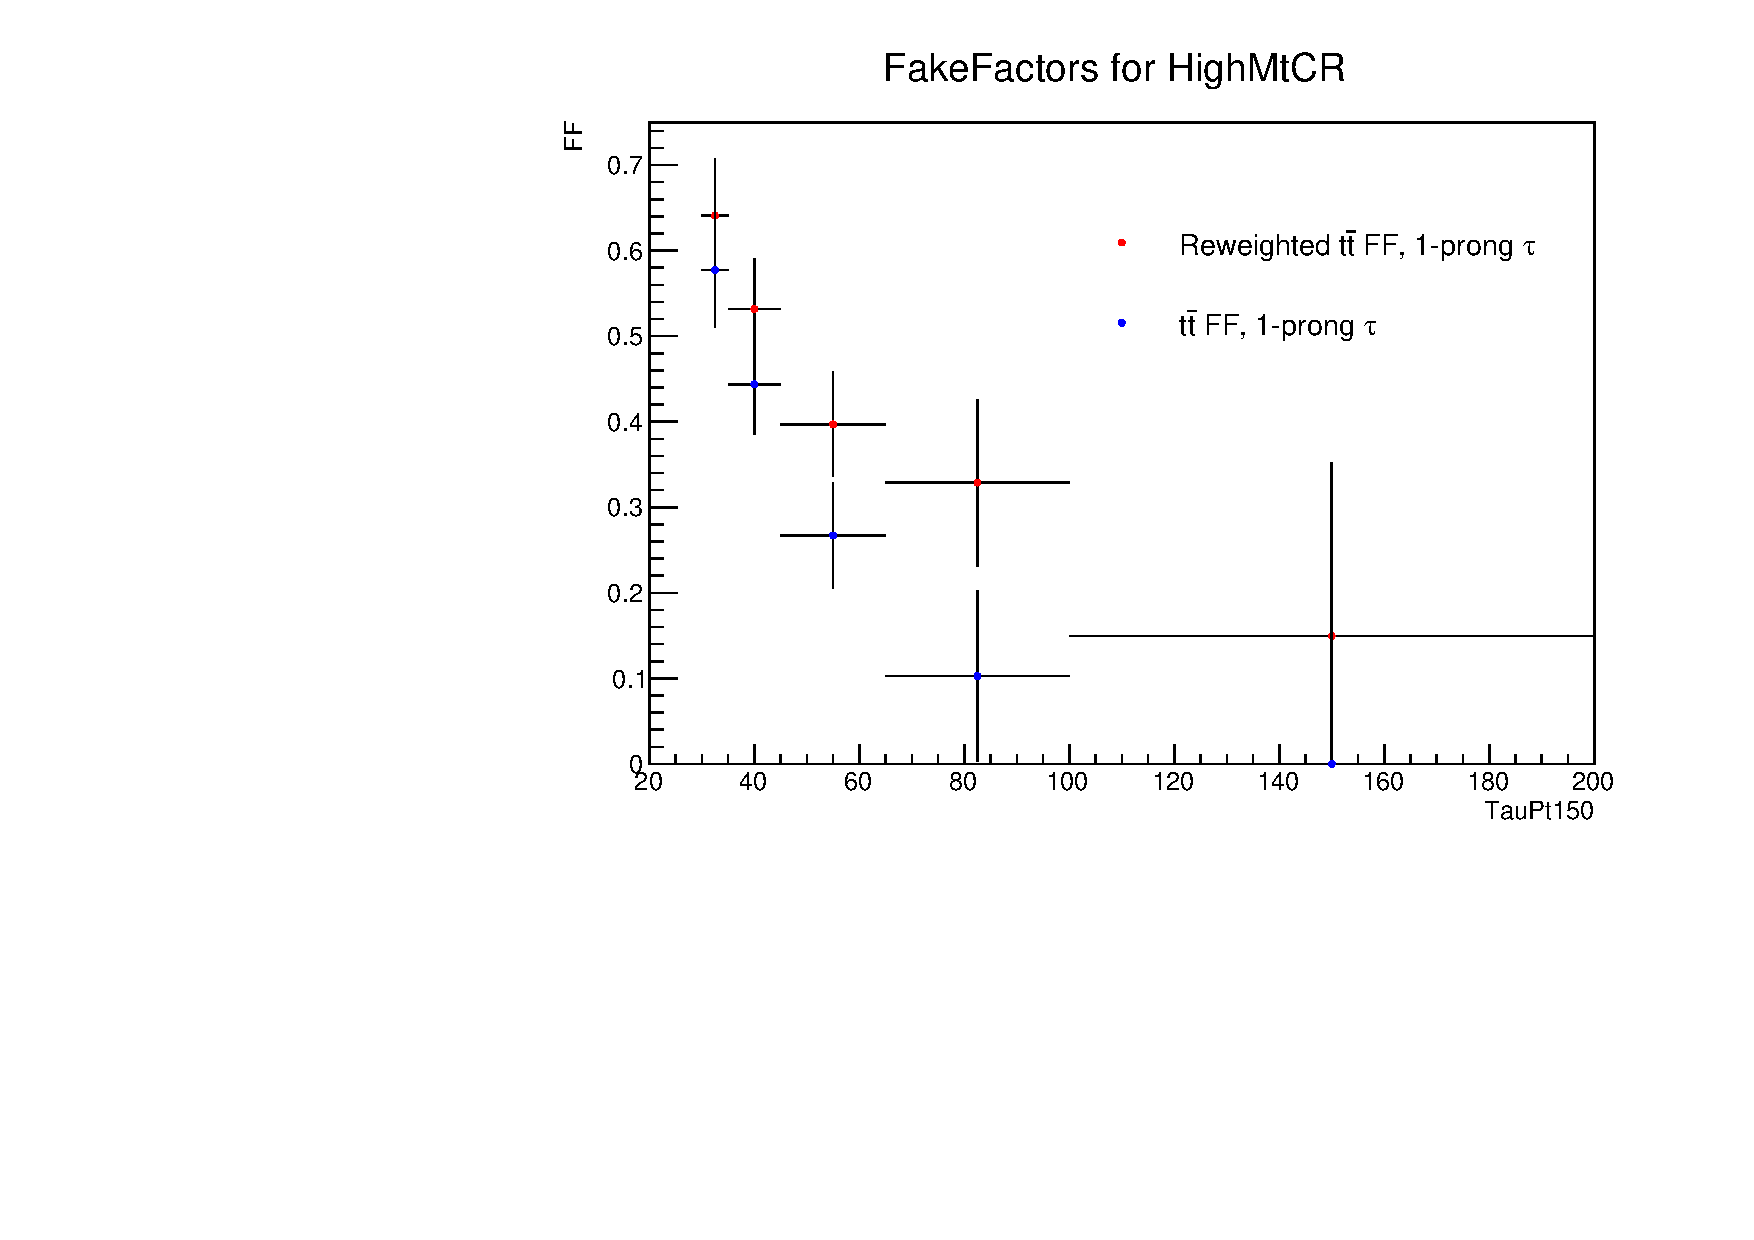
\includegraphics[width=.45\textwidth]{figures/systs/datadriven_lephadfakes/LTT/FFRWUnc_1prong_LTT.pdf}
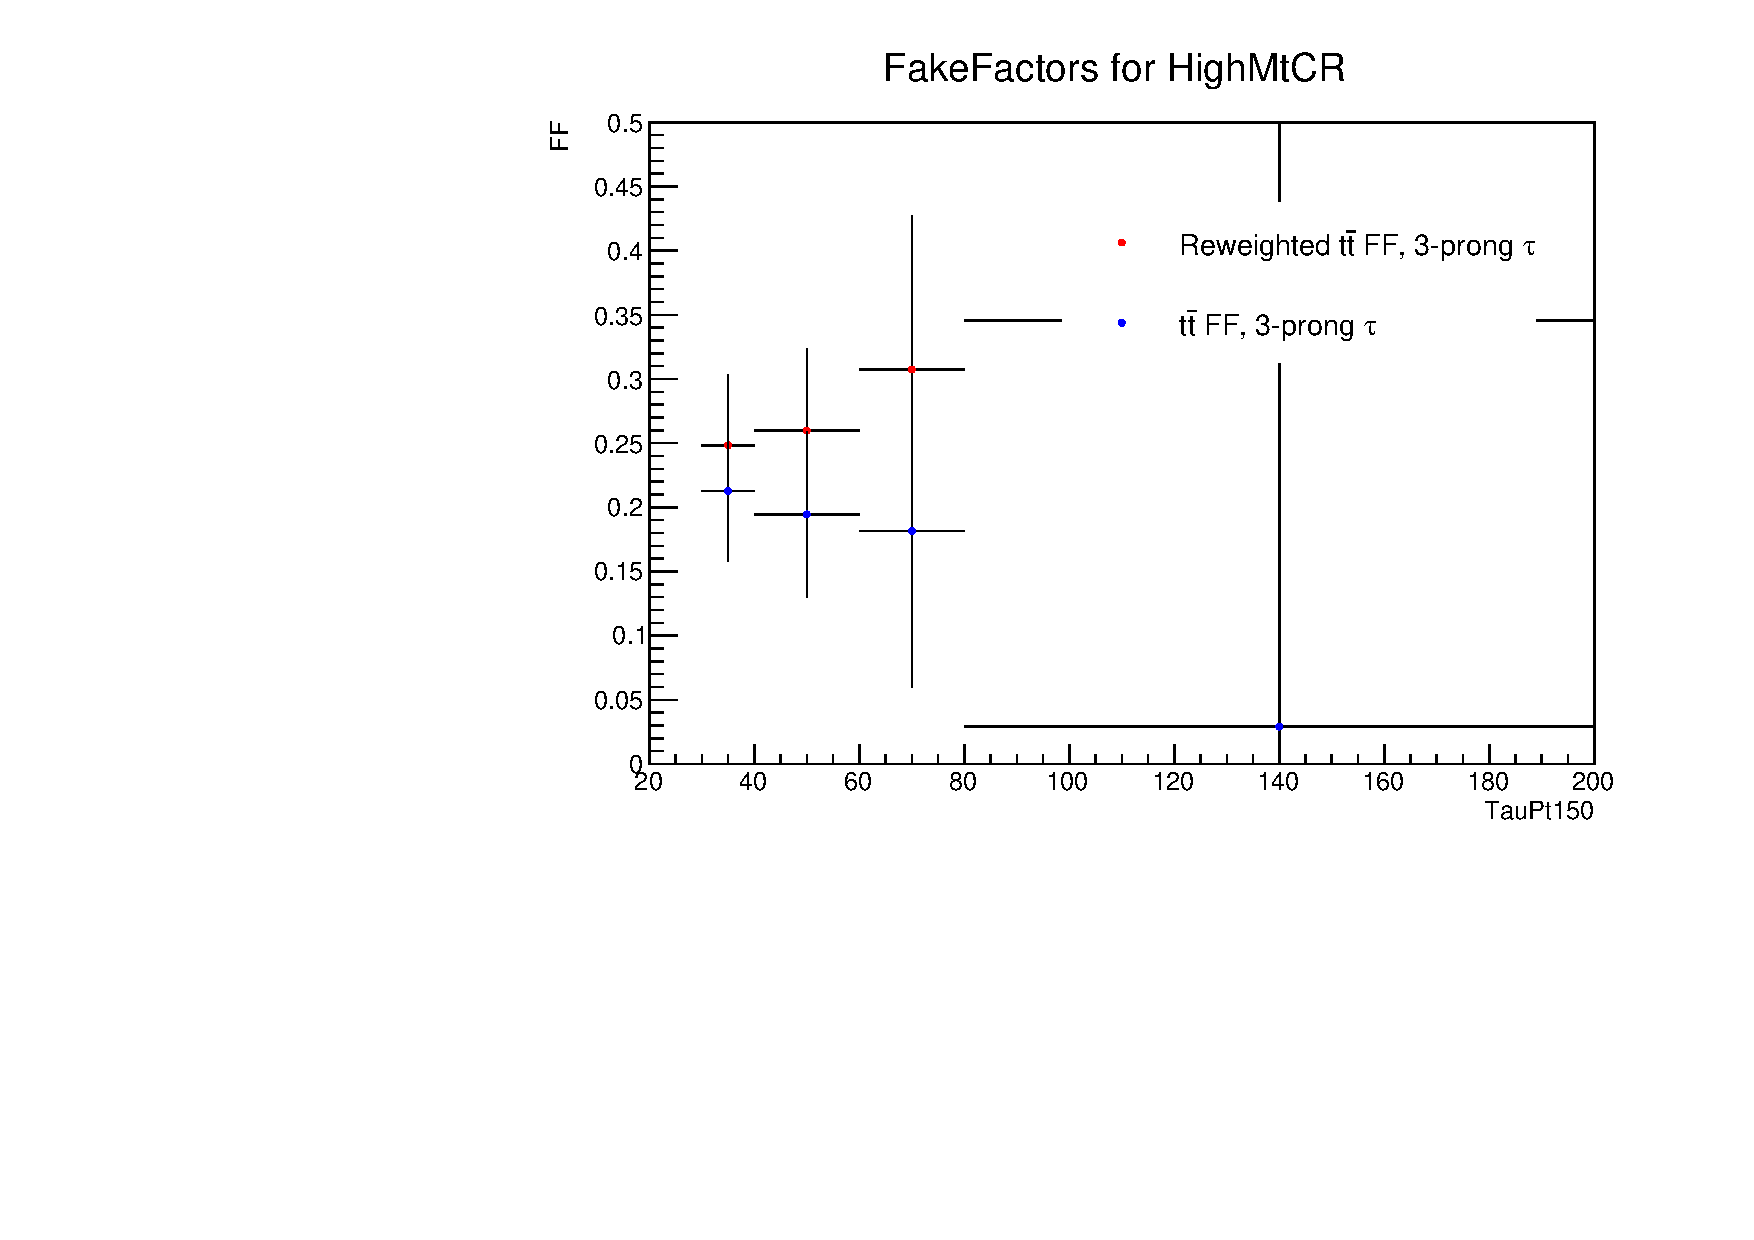
\includegraphics[width=.45\textwidth]{figures/systs/datadriven_lephadfakes/LTT/FFRWUnc_3prong_LTT.pdf} \\
\caption{Fake-factors for 1-prong (left) and 3-prong (right) \tauhad candidates for \ttbar process with and without applying \ttbar reweighting, shown for both the \lephad SLT (top) and the \lephad LTT (bottom) categories.}
\label{fig:FFRW}
\end{figure}

An additional uncertainty on the extrapolation of the $t\bar{t}$ fake factors from the high $M_{bb}$ region to the low $M_{bb}$ region was also considered, using simulation to evaluate the level of non-closure.  No systematic difference was observed, so this will not be included as an uncertainty.
